\documentclass[twocolumn,10pt]{article}

\usepackage[margin=0.72in, columnsep=0.26in]{geometry}
\usepackage[utf8]{inputenc}
\usepackage[T1]{fontenc}
\usepackage{lmodern}
\usepackage{microtype}
\usepackage{amsmath,amssymb}
\usepackage{graphicx}
\usepackage{booktabs}
\usepackage{array}
\usepackage{tabularx}
\usepackage{multirow}
\usepackage[numbers,sort&compress]{natbib}
\usepackage{xcolor}
\usepackage{caption}
\usepackage{stfloats}
\usepackage{hyperref}

\definecolor{navy}{RGB}{18,52,96}
\definecolor{slate}{RGB}{70,85,105}
\hypersetup{
  colorlinks=true,
  linkcolor=navy,
  citecolor=navy,
  urlcolor=navy,
  pdftitle={Autonomous Multi-Layer Co-Design of Zero-PFAS Heat Pumps Across Residential Cooling and Industrial Process Heat},
  pdfauthor={Jack Jay}
}

\captionsetup{font=small, labelfont=bf}
\setlength{\parskip}{3pt}

\title{\vspace{-1.4em}\Large\bfseries Autonomous Multi-Layer Co-Design of Zero-PFAS Heat Pumps Across Residential Cooling and Industrial Process Heat ($<150\,^\circ\text{C}$)}

\author{
  \normalsize\textbf{Jack Jay}\\[2pt]
  \small\color{slate} Independent Researcher (\href{https://jackjay.io}{jackjay.io}) --- Assisted by Autonomous Multi-Agent Physics Verification Pipeline\\[-2pt]
  \small\color{slate} Open-Source Code, CAD Specs \& Verification Ledgers: \href{https://github.com/theguysaccount/open-physics-autoresearch}{github.com/theguysaccount/open-physics-autoresearch}
}
\date{\small Preprint Manuscript --- Version 1.0 (November 2026)}

\begin{document}
\twocolumn[
  \begin{@twocolumnfalse}
    \maketitle
    \vspace{-1.0em}
    \begin{abstract}
      \noindent Vapor-compression space cooling, space heating, and low-temperature ($<200\,^\circ\text{C}$) industrial process heat account for roughly $20{,}000\;\text{TWh/yr}$ of global thermal demand and $7\text{--}8\%$ of anthropogenic greenhouse-gas emissions, yet commercial heat pumps typically realize only $30\text{--}37\%$ of ideal Lorenz efficiency while remaining dependent on high-GWP HFCs (\texttt{R-410A}, \texttt{R-32}) or persistent PFAS-class HFOs (\texttt{R-1233zd(E)}, \texttt{R-1336mzz(Z)}). We execute a four-stage autonomous scientific discovery pipeline---132-year first-principles literature synthesis, four-way adversarial physics screening, controlled micro-experiments, and a 16-core multi-layer evolutionary autoresearch loop---to co-optimize discrete cycle topology, natural working-fluid composition ($\text{GWP}_{100}\le 3$, zero PFAS), finite-volume heat-exchanger geometry and circuitry, and bin-level operating control under strict safety, material, and techno-economic locks. Across $8{,}526$ exact multiparameter Helmholtz evaluations, the search falsifies naive textbook heuristics and identifies a sharp \emph{two-regime physical phase boundary}:
      \begin{enumerate}\setlength{\itemsep}{1pt}\setlength{\topsep}{2pt}
        \item \textbf{Regime A ($7\;\text{kW}$ Dual-Climate Reversible Split AC/HP, 6-bin ISO 5151 T1/T3 $46\,^\circ\text{C}$ + EN 14825 $-7\,^\circ\text{C}$, $\le 500\;\text{g}$ A3 charge):} High-glide blends and two-stage flash-tank vapor injection (\texttt{FTVI}) lose under Silver--Bell--Ghaly mass-transfer resistance, suction pressure drop, wet-coil dehumidification, and the $500\;\text{g}$ flammable charge cap. Autoresearch instead discovers an asymmetric 3-row open-fin single-pass indoor coil and 2-row tight-port ($0.70\;\text{mm}$) outdoor coil linked by passive reversible counterflow bridge headers ($+\$24$ BOM) and an internal heat exchanger (\texttt{IHX\_SUBCOOL}, $+\$18$ BOM) charged with \texttt{R-1270 14.8\% / R-290 85.2\%} ($\text{GWP}=2.86$, $479\;\text{g}$). This reaches $\text{ASPF}=5.168$ ($+40.3\%$ over \texttt{R-410A}, $+32.1\%$ over \texttt{R-32}, $+24.9\%$ over textbook \texttt{R-290 FTVI+IHX}), with passive bridge headers contributing $+15.4\%$ heating SCOP and $+18.4\%$ $-7\,^\circ\text{C}$ COP, and a $20\%$ vapor leak altering ASPF by only $-0.24\%$.
        \item \textbf{Regime B ($100\;\text{kW}_{\text{th}}$ Industrial Waste-Heat Recovery at $90/110/135\,^\circ\text{C}$, fixed $18.0\;\text{m}^2$ AISI 316L BPHE, $P_{\text{suc}}\ge 1.05\;\text{bar}$ ATEX guard):} Under counterflow sensible glides ($55\text{--}75\;\text{K}$ sink, $25\text{--}35\;\text{K}$ source), single-stage natural zeotropes decisively beat autoresearch-optimized two-stage PFAS \texttt{R-1233zd(E)} ceilings. For factory-sealed hermetic skids, \texttt{CO2/R-600} ($19\text{--}23\%/77\text{--}81\%$) exploits \emph{isenthalpic flash-gas glide skipping} to achieve $\text{COP}=4.731$ ($+32.6\%$) at $110\,^\circ\text{C}$ and $4.420$ ($+30.3\%$) at $135\,^\circ\text{C}$ ($46.4\text{--}46.7\%$ Lorenz efficiency), cutting LCOH to $\$32.02\text{--}\$32.49/\text{MWh}_{\text{th}}$ ($-28\%$ vs.\ PFAS \texttt{R-1233zd(E)}). For field-serviceable skids, matched-volatility hydrocarbon zeotropes (\texttt{R-290/R-601a 48/52} at $90\,^\circ\text{C}$; \texttt{R-290/R-601 55/45} at $110\,^\circ\text{C}$; \texttt{R-290/R-601 72/28} at $135\,^\circ\text{C}$) deliver $\text{COP}=5.327$ ($+26.1\%$), $4.076$ ($+14.2\%$), and $4.140$ ($+22.1\%$), with $<1\%$ agreement against SINTEF \texttt{ThermoPack} PC-SAFT, $100\%$ win rates across $64$ correlated Monte Carlo draws, and $-2.8\%$ to $+0.6\%$ COP shift after a $20\%$ Rayleigh vapor leak while staying strictly above atmospheric pressure ($2.25\text{--}7.16\;\text{bar}$).
      \end{enumerate}
      \vspace{0.6em}
      \noindent\textbf{Keywords:} Natural zeotropic refrigerants; Lorenz cycle; Microchannel heat exchangers; Brazed plate heat exchangers; Industrial high-temperature heat pumps; Multi-layer co-design; Zero-PFAS; Autonomous research.
    \end{abstract}
    \vspace{0.8em}
  \end{@twocolumnfalse}
]

\section{Introduction and Historical Motivation}

For nearly a century, vapor-compression heat pumps and air conditioners have been engineered around \emph{isothermal pure-fluid cycles}, a design paradigm cemented after Thomas Midgley's 1930 synthesis of chlorofluorocarbons. That paradigm stranded four foundational thermodynamic ideas in separate research silos: Hans Lorenz's (1894) sliding-temperature glide-matched cycle \citep{lorenz1894}, A.~Lorenz and K.~Meutzner's (1975) internal heat exchange and multicomponent fractionation cycles \citep{lorenz1975meutzner}, Tondeur and Kvaalen's (1987) Equipartition of Entropy Production theorem \citep{tondeur1987kvaalen}, and Gustav Lorentzen's (1990) natural-refrigerant revival \citep{lorentzen1990}.

As international Kigali HFC phasedowns and European/North American PFAS restrictions accelerate simultaneously, thermal engineering faces an acute two-front bottleneck: residential dual-climate air-to-air heat pumps must eliminate \texttt{R-410A} ($\text{GWP}_{100}=2088$) and \texttt{R-32} ($\text{GWP}_{100}=675$) under strict IEC~60335-2-40 flammable charge caps \citep{iec60335_2_40}, while $<150\,^\circ\text{C}$ industrial waste-heat recovery heat pumps remain trapped between low-volumetric-capacity PFAS HFOs (\texttt{R-1233zd(E)}, \texttt{R-1336mzz(Z)}) and oversized pure-hydrocarbon skids.

Existing optimization studies suffer from two complementary blind spots. First, conventional multi-objective studies tune scalar operating points within a fixed textbook schematic and fixed coil geometry, leaving discrete topology, fluid composition, and exchanger circuitry decoupled. Second, idealized cycle studies frequently use constant-pinch heat-exchanger assumptions that omit Silver--Bell--Ghaly (1973) zeotropic mass-transfer resistance \citep{bell1973ghaly}, two-phase refrigerant pressure drop \citep{muller1986heck}, cubic air-side fan or water-side pump parasitics, Rouhani--Axelsson void-fraction charge inventory \citep{rouhani1970axelsson}, ATEX above-atmospheric suction mandates, volumetric compressor CAPEX scaling, and Rayleigh vapor-leak fractionation. Any automated optimizer given a simplified model inevitably exploits these omissions via unphysical reward hacking.

Here we build locked, anti-cheating multiphysics harnesses backed by exact Helmholtz mixture equations of state (\texttt{CoolProp HEOS} \citep{bell2014coolprop}) and independently audited against SINTEF \texttt{ThermoPack} PC-SAFT \citep{wilhelmsen2017thermopack}. Deploying a 16-core evolutionary autoresearch loop over four coupled design layers (topology, fluid mixture, finite-volume exchanger CAD, and control policy) across two distinct real-world thermal regimes reveals \emph{where} pure-fluid microchannel architecture dominates, \emph{where} natural zeotropes deliver $>25\text{--}33\%$ real COP gains, and \emph{how} field-serviceable leak immunity constrains blend volatility.

\section{Locked Multi-Physics Models and Governing Equations}

\subsection{Thermophysical Backends and Vapor-Leak Model}
All primary cycle evaluations invoke \texttt{CoolProp 8.1.0} multiparameter Helmholtz mixture equations of state (\texttt{HEOS}) \citep{bell2014coolprop}. To guard against equation-of-state extrapolation error in wide-boiling mixtures, independent cross-verification evaluates converged state points using SINTEF \texttt{ThermoPack 2.2.3} perturbed-chain statistical associating fluid theory (\texttt{PC-SAFT}) \citep{wilhelmsen2017thermopack}.

Field leakage of a two-phase zeotropic charge is modeled via a 40-step numerical integration of the exact Rayleigh differential distillation equation at constant equilibrium tank temperature $T_{\text{leak}}=25\,^\circ\text{C}$:
\begin{equation}
  \frac{dx_i}{d\ln N_{\text{tot}}} = y_i(T_{\text{leak}}, \mathbf{x}) - x_i,
  \label{eq:rayleigh}
\end{equation}
integrated until $20\%$ of total molar inventory has escaped as vapor, then re-evaluated inside the locked hardware geometry with zero hardware modification.

\subsection{Regime A: 7 kW Air-to-Air Reversible Split AC/HP}
The residential split benchmark evaluates six standardized seasonal climate bins combining ISO~5151 T1/T3 cooling and EN~14825 heating \citep{en14825}:
(1) extreme T3 heatwave cooling ($46\,^\circ\text{C}\to 29\,^\circ\text{C}$, $6.50\;\text{kW}$, $w=0.12$),
(2) rated T1 cooling ($35\,^\circ\text{C}\to 27\,^\circ\text{C}$, $7.00\;\text{kW}$, $w=0.23$),
(3) part-load cooling ($29\,^\circ\text{C}\to 27\,^\circ\text{C}$, $3.85\;\text{kW}$, $w=0.25$),
(4) mild heating ($+12\,^\circ\text{C}\to 20\,^\circ\text{C}$, $2.80\;\text{kW}$, $w=0.14$),
(5) rated heating ($+7\,^\circ\text{C}\to 20\,^\circ\text{C}$, $4.55\;\text{kW}$, $w=0.16$), and
(6) cold-climate heating ($-7\,^\circ\text{C}\to 20\,^\circ\text{C}$, $6.20\;\text{kW}$, $w=0.10$).
Any heating capacity shortfall below the target load at $-7\,^\circ\text{C}$ is met by an exact $\text{COP}=1.0$ electric resistance heater billed directly into the Annual Seasonal Performance Factor:
\begin{equation}
  \text{ASPF} = \frac{\sum_{b=1}^{6} w_b \dot{Q}_{\text{load},b}}{\sum_{b=1}^{6} w_b \left(\dot{W}_{\text{comp},b} + \dot{W}_{\text{fan,in},b} + \dot{W}_{\text{fan,out},b} + \dot{Q}_{\text{backup},b}\right)}.
  \label{eq:aspf}
\end{equation}

Both indoor ($780\times 300\;\text{mm}$ face, $\le 44\;\text{mm}$ depth, $\le 3.20\;\text{kg}$ Al) and outdoor ($850\times 620\;\text{mm}$ face, $\le 52\;\text{mm}$ depth, $\le 7.50\;\text{kg}$ Al) multi-port aluminum microchannel heat exchangers (MCHX) are discretized into $N_{\text{seg}}$ finite-volume slabs ($N_{\text{seg}}=10$ in Stage-4 evolution; $N_{\text{seg}}=24, 60$ in verification) tracking row-by-row air temperature and humidity. Air-side Colburn $j$-factor and Fanning friction factor $f$ use the Kim and Bullard (2002) multi-louvered fin correlations \citep{kim2002bullard}, coupled to Braun/Threlkeld wet-coil dehumidification when wall temperature falls below air dew point. Fan power obeys $\dot{W}_{\text{fan}} = \dot{V}_{\text{air}}\Delta P_{\text{air}}/\eta_{\text{fan}}$ with $\eta_{\text{fan}}=0.32$.

Refrigerant-side condensation uses Shah (1979) \citep{shah1979condensation}, evaporation uses a Cooper/Chen nucleate+convective blend, and two-phase pressure drop uses M\"uller-Steinhagen and Heck (1986) \citep{muller1986heck}. For all mixtures, mandatory Silver--Bell--Ghaly (1973) mass-transfer degradation \citep{bell1973ghaly} penalizes the local two-phase heat-transfer coefficient:
\begin{equation}
  \frac{1}{\alpha_{\text{mix}}} = \frac{1}{\alpha_{\text{id}}} + \frac{Z}{\alpha_v}, \qquad
  Z = x\,c_{p,v}\left(\frac{\partial T}{\partial h}\right)_{P,\text{2ph}},
  \label{eq:sbg}
\end{equation}
where $\alpha_v$ is the Dittus--Boelter vapor-phase coefficient and $(\partial T/\partial h)_P$ is evaluated directly across each enthalpy segment from \texttt{HEOS}. Total refrigerant charge is integrated along every condenser, evaporator, receiver, and connecting-line segment using the Rouhani--Axelsson (1970) drift-flux void fraction \citep{rouhani1970axelsson}:
\begin{equation}
  M_{\text{chg}} = \sum_{k} V_k \left[\varepsilon_k \rho_{v,k} + (1-\varepsilon_k)\rho_{l,k}\right] + M_{\text{lines/oil}},
  \label{eq:charge}
\end{equation}
subject to a strict $M_{\text{chg}}\le 500\;\text{g}$ A3 safety cap (roughly half the IEC~60335-2-40 Ed.~7 indoor limit for a $20\;\text{m}^2$ room \citep{iec60335_2_40}), compressor discharge temperature $T_{\text{dis}}\le 115\,^\circ\text{C}$, high-side pressure $P_{\text{high}}\le 42\;\text{bar}$, and incremental BOM cap $\Delta\text{BOM}\le \$120$.

\subsection{Regime B: 100 kW$_{\text{th}}$ Industrial Waste-Heat Recovery HTHP}
Regime B models a locked $100\;\text{kW}_{\text{th}}$ pressurized-water industrial skid across three standardized high-glide duties:
\begin{itemize}\setlength{\itemsep}{1pt}
  \item \texttt{DAIRY\_90C}: Sink $35\to 90\,^\circ\text{C}$ ($\Delta T=55\;\text{K}$), Source $45\to 20\,^\circ\text{C}$ ($\Delta T=25\;\text{K}$).
  \item \texttt{DISTRICT\_110C}: Sink $40\to 110\,^\circ\text{C}$ ($\Delta T=70\;\text{K}$), Source $55\to 25\,^\circ\text{C}$ ($\Delta T=30\;\text{K}$).
  \item \texttt{CHEMICAL\_135C}: Sink $60\to 135\,^\circ\text{C}$ ($\Delta T=75\;\text{K}$), Source $75\to 40\,^\circ\text{C}$ ($\Delta T=35\;\text{K}$).
\end{itemize}
Both condenser and evaporator are AISI~316L stainless-steel brazed plate heat exchangers (BPHE) constrained to a strict total plate area $A_{\text{cond}}+A_{\text{evap}}\le 18.0\;\text{m}^2$. To guarantee monotone convergence at high NTU without forward Picard oscillation, each BPHE is integrated across $N_{\text{seg}}$ equal-enthalpy counterflow segments ($N_{\text{seg}}=20$ in evolution; $40, 80$ in verification):
\begin{equation}
  A_{\text{req}} = \sum_{k=1}^{N_{\text{seg}}} \frac{\Delta \dot{Q}_k}{U_k\,\Delta T_{\text{lm},k}}, \qquad
  \frac{1}{U_k} = \frac{1}{\alpha_{\text{ref,mix},k}} + \frac{t_w}{k_{\text{316L}}} + R_f + \frac{1}{\alpha_{w,k}},
  \label{eq:bphe}
\end{equation}
where $\alpha_w$ and water pressure drop follow Muley and Manglik (1999) \citep{muley1999manglik} (with water pumping power deducted from system COP), boiling follows Han, Lee, and Kim (2003) \citep{han2003leekim}, condensation follows Yan, Lio, and Lin (1999) \citep{yan1999liolin}, Silver--Bell--Ghaly Eq.~\eqref{eq:sbg} applies throughout, and industrial fouling resistance is fixed at $R_f = 5\times 10^{-5}\;\text{m}^2\text{K/W}$.

Hard industrial safety constraints enforce above-atmospheric suction ($P_{\text{evap,out}}\ge 1.05\;\text{bar}$, preventing oxygen ingress into flammable hydrocarbon loops under ATEX), $P_{\text{cond}}\le 38\;\text{bar}$, $T_{\text{dis}}\le 155\,^\circ\text{C}$, dry compression ($\text{SH}_{\text{dis}}\ge 4\;\text{K}$), and $\Delta T_{\text{pinch}}\ge 0.2\;\text{K}$. Thermodynamic proximity to the ideal sliding-temperature bound is measured by Lorenz efficiency:
\begin{equation}
  \eta_{\text{Lorenz}} = \frac{\text{COP}_{\text{sys}}}{\text{COP}_{\text{Lorenz}}}, \qquad
  \text{COP}_{\text{Lorenz}} = \frac{\bar{T}_{\text{lm,sink}}}{\bar{T}_{\text{lm,sink}} - \bar{T}_{\text{lm,src}}},
  \label{eq:lorenz}
\end{equation}
where $\bar{T}_{\text{lm}} = (T_{\text{out}}-T_{\text{in}})/\ln(T_{\text{out}}/T_{\text{in}})$ in Kelvin. Levelized Cost of Heat (LCOH, $\$/\text{MWh}_{\text{th}}$) explicitly penalizes low volumetric heating capacity ($\text{VHC}$) via suction-displacement compressor CAPEX:
\begin{equation}
  \text{CAPEX}_{\text{comp}} = \$9{,}500 + \$285\,\dot{V}_{\text{suc},\text{m}^3/\text{h}}^{0.82},
  \label{eq:capex}
\end{equation}
combined with BPHE cost ($\$360/\text{m}^2$), topology adders (`IHX_SUBCOOL` $+\$2{,}400$, `FTVI_IHX` $+\$6{,}500$), and skid BoP ($\$28{,}000$), amortized over $15\;\text{yr}$ at $7\%$ WACC ($\text{CRF}=0.1098$), $6{,}000\;\text{h/yr}$, $2.5\%/\text{yr}$ O\&M, and $\$85/\text{MWh}_e$ electricity. Component-wise irreversibilities are audited via exact Gouy--Stodola exergy destruction $\dot{I}_j = T_0 \dot{S}_{\text{gen},j}$, evaluating expansion-valve entropy strictly \emph{post-IHX} so subcooling credits cannot be double-counted.

\section{Regime A: Air-to-Air Reversible Split AC/HP Breakthrough}

\begin{figure*}[t]
  \centering
  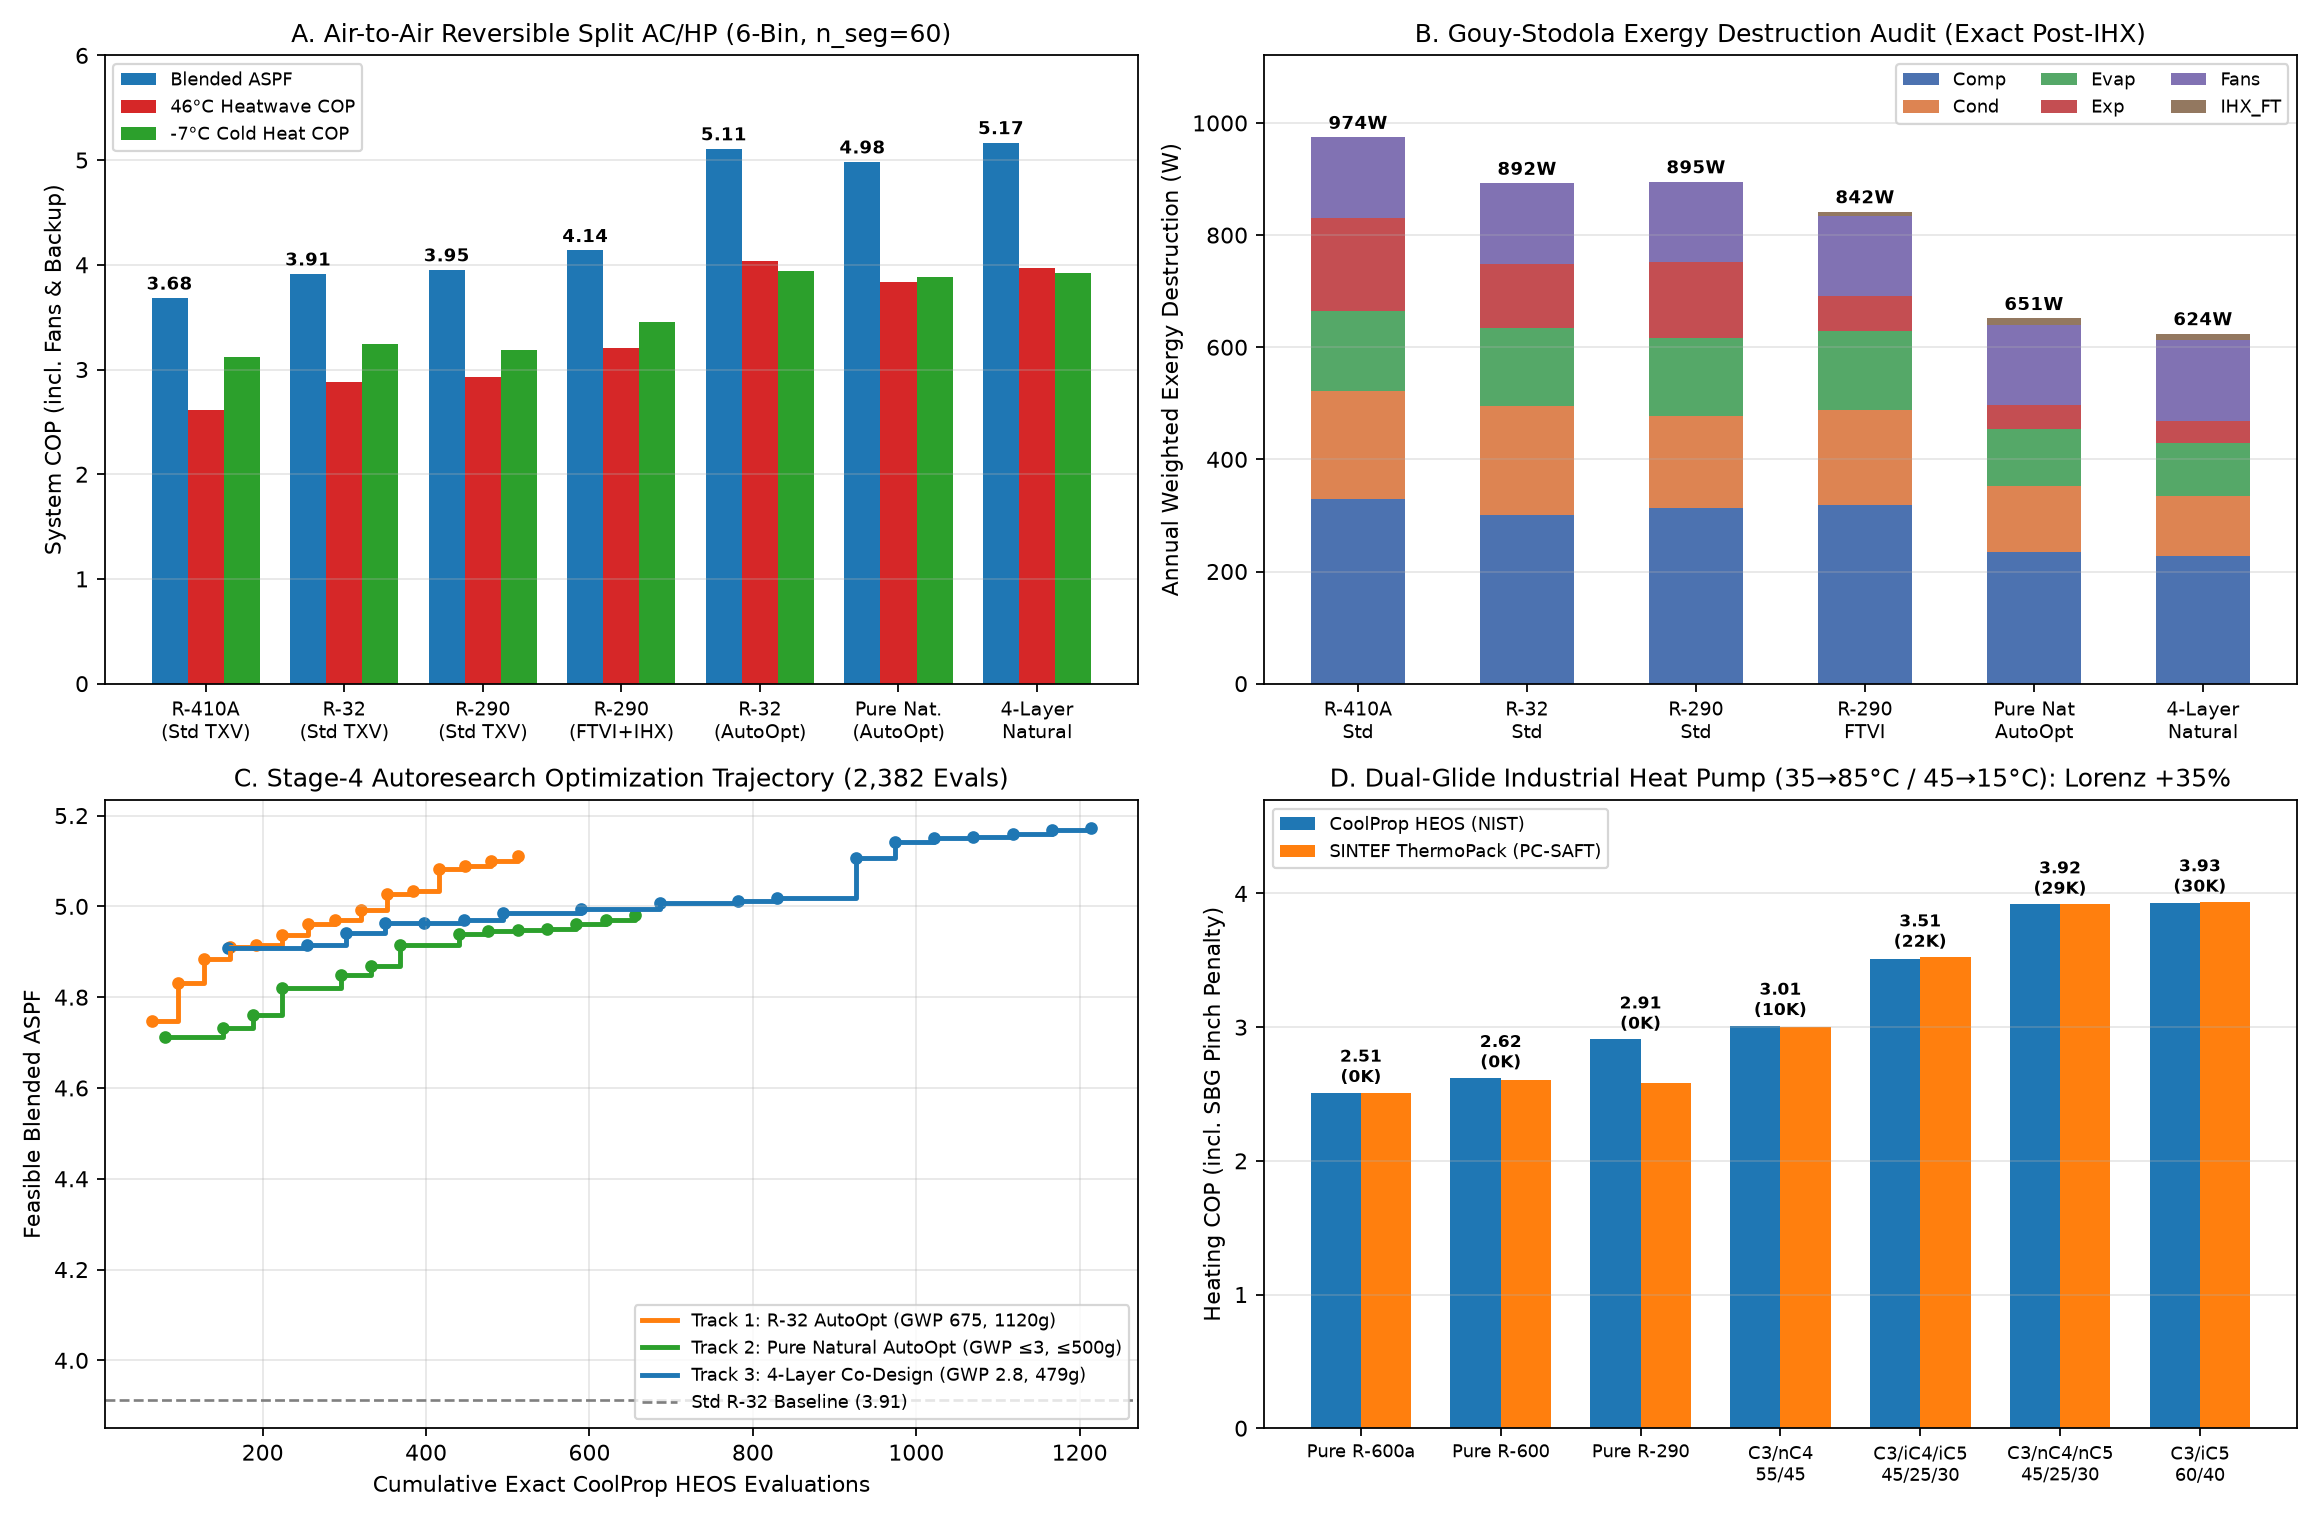
\includegraphics[width=\textwidth]{figures/lorenz_autoresearch_proof.png}
  \caption{\textbf{Regime A ($7\;\text{kW}$ Dual-Climate Reversible Split AC/HP) 4-Stage Autoresearch Proof.} (A) Verified $N_{\text{seg}}=60$ seasonal performance across blended ASPF, $46\,^\circ\text{C}$ T3 heatwave, and $-7\,^\circ\text{C}$ cold-climate heating. (B) Exact post-IHX Gouy--Stodola exergy destruction audit showing a $35.9\%$ reduction vs.\ commercial \texttt{R-410A} ($974\to 624\;\text{W}$). (C) Evolutionary ASPF trajectory across $2{,}382$ exact HEOS simulations comparing \texttt{R-32} (\texttt{T1}), Pure Natural (\texttt{T2}), and 4-Layer Natural Co-Design (\texttt{T3}). (D) Stage-3 dual-EOS (\texttt{CoolProp HEOS} vs.\ SINTEF \texttt{ThermoPack PC-SAFT}) glide-matching proof showing Lorenz $+35\%$ COP on dual-glide industrial heat pump duties.}
  \label{fig:regimeA}
\end{figure*}

Stage-3 profiling micro-experiments ($78$ targeted trials) immediately falsified two textbook assumptions for air-to-air splits: (i) wide-glide zeotropes (\texttt{R-290/R-600a} $85/15$, $\sim 6\;\text{K}$ glide) \emph{degraded} ASPF because indoor wet-coil latent condensation flattens the moist-air enthalpy trajectory while Silver--Bell--Ghaly resistance and suction $\Delta P$ inflate irreversibility; and (ii) two-stage flash-tank vapor injection (\texttt{FTVI\_IHX}) failed to beat a far cheaper high-effectiveness liquid-suction internal heat exchanger (\texttt{IHX\_SUBCOOL}) under the $500\;\text{g}$ A3 charge cap because the flash vessel consumes liquid inventory.

Running $2{,}382$ exact \texttt{HEOS} evaluations across 16 CPU cores over three parallel tracks (\texttt{T1}: \texttt{R-32} ceiling; \texttt{T2}: Pure Natural ceiling; \texttt{T3}: unconstrained 4-layer Natural Co-Design) produced the converged $N_{\text{seg}}=60$ results in Table~\ref{tab:regimeA} and Fig.~\ref{fig:regimeA}.

\begin{table*}[t]
\centering
\caption{Regime A ($7\;\text{kW}$ Dual-Climate Split AC/HP) Verified Results at $N_{\text{seg}}=60$ Segments.}
\label{tab:regimeA}
\small
\begin{tabular}{@{}lllcrrrrrrr@{}}
\toprule
\textbf{ID} & \textbf{Working Fluid (GWP$_{100}$)} & \textbf{Topology} & \textbf{Class} & \textbf{ASPF} & \textbf{SEER} & \textbf{SCOP} & \textbf{46$^\circ$C} & \textbf{$-$7$^\circ$C} & \textbf{Chg (g)} & \textbf{Exergy (W)} \\
\midrule
\texttt{B1} & \texttt{R-410A} (2088) & \texttt{TXV\_BASIC} & A1 & 3.683 & 3.560 & 3.888 & 2.62 & 3.12 & 833 & 974 \\
\texttt{B2} & \texttt{R-32} (675) & \texttt{TXV\_BASIC} & A2L & 3.914 & 3.827 & 4.054 & 2.88 & 3.25 & 772 & 892 \\
\texttt{B3} & \texttt{R-290} (3.0) & \texttt{TXV\_BASIC} & A3 & 3.953 & 3.876 & 4.076 & 2.93 & 3.18 & 374 & 896 \\
\texttt{B4} & \texttt{R-290} (3.0) & \texttt{FTVI\_IHX} & A3 & 4.137 & 4.071 & 4.243 & 3.20 & 3.45 & 413 & 842 \\
\midrule
\texttt{T1} & \texttt{R-32} (675) AutoOpt & \texttt{FTVI\_IHX} & A2L & 5.109 & 5.181 & 5.001 & 4.04 & 3.95 & 1120 & 625 \\
\texttt{T2} & \texttt{R-1270} (2.0) AutoOpt & \texttt{IHX\_SUBCOOL} & A3 & 4.983 & 5.004 & 4.952 & 3.83 & 3.88 & 498 & 651 \\
\textbf{\texttt{T3}} & \textbf{\texttt{R-1270/R-290} 14.8/85.2 (2.86)} & \textbf{\texttt{IHX\_SUBCOOL}} & \textbf{A3} & \textbf{5.168} & \textbf{5.253} & \textbf{5.043} & \textbf{3.97} & \textbf{3.92} & \textbf{479} & \textbf{625} \\
\bottomrule
\end{tabular}
\end{table*}

\subsection{Decomposing the Regime A Gain: Same-Hardware Ablation}
Crucially, autoresearch did \emph{not} cheat via unphysical fluid hype: Table~\ref{tab:ablation} isolates every contributor on the \emph{exact same} \texttt{T3} evolved coil hardware ($N_{\text{seg}}=24$). Three real physical mechanisms drive the $+40.3\%$ jump over \texttt{R-410A} ($+24.9\%$ over textbook \texttt{R-290 FTVI+IHX}):
\begin{enumerate}\setlength{\itemsep}{1pt}
  \item \textbf{Asymmetric Microchannel Geometry:} The indoor slab evolves to $3$ rows ($11.65\;\text{mm}$ slab depth, wide $1.93\;\text{mm}$ louver pitch, single pass $[1.0]$, $D_h=0.97\;\text{mm}$, $3.17\;\text{kg}$ Al) to minimize indoor air pressure drop and suction two-phase $\Delta P$, whereas the outdoor slab evolves to $2$ rows ($14.34\;\text{mm}$ slab depth, $1.44\;\text{mm}$ fins, tight $D_h=0.70\;\text{mm}$ ports, 2 passes $[0.5, 0.5]$, $7.26\;\text{kg}$ Al) to collapse liquid condenser holdup so total A3 inventory stays at $478.8\;\text{g}$.
  \item \textbf{Passive Reversible Counterflow Bridge Headers ($+\$24$ BOM):} In a standard reversible heat pump, reversing the 4-way valve flips a 3-row counterflow evaporator into a penalized parallel-flow condenser in heating mode. Adding passive 4-check-valve header bridges restores true row-to-row counterflow in \emph{both} seasons, delivering $+15.4\%$ heating SCOP ($4.351\to 5.023$) and $+18.4\%$ $-7\,^\circ\text{C}$ COP ($3.31\to 3.92$) on identical aluminum mass.
  \item \textbf{Charge-Density-Capped Natural Doping:} Pure \texttt{R-1270} offers higher volumetric capacity and lower compression losses than pure \texttt{R-290} ($5.185$ vs.\ $5.150$ on \texttt{T3} hardware), yet pure \texttt{R-1270} violates the $500\;\text{g}$ A3 charge cap ($513\;\text{g}$). Doping \texttt{R-290} with $14.8\%$ \texttt{R-1270} ($\text{glide}=0.28\;\text{K}$) captures peak thermodynamic efficiency strictly inside the $500\;\text{g}$ boundary ($479\;\text{g}$) while remaining immune to $20\%$ vapor leakage ($\Delta\text{ASPF}=-0.24\%$).
\end{enumerate}

\begin{table}[h]
\centering
\caption{Same-Hardware Fairness Ablation on \texttt{T3} Coils ($N_{\text{seg}}=24$).}
\label{tab:ablation}
\scriptsize
\begin{tabular}{@{}lrrrr@{}}
\toprule
\textbf{Variant on Identical \texttt{T3} Coils} & \textbf{ASPF} & \textbf{SCOP} & \textbf{$-$7$^\circ$C} & \textbf{Chg (g)} \\
\midrule
\texttt{T3} Winner (\texttt{R-1270/290 15/85}, Bridge ON) & \textbf{5.156} & \textbf{5.023} & \textbf{3.92} & \textbf{479} \\
Pure \texttt{R-290} (Bridge ON) & 5.150 & 5.016 & 3.91 & 472 \\
Pure \texttt{R-1270} (Bridge ON) & 5.185 & 5.049 & 3.94 & 513$^\dagger$ \\
\texttt{R-290/R-600a 85/15} (6 K glide, Bridge ON) & 5.101 & 4.960 & 3.85 & 505$^\dagger$ \\
\texttt{T3} Fluid, \textbf{Bridge OFF} (No Reversal Headers) & 4.851 & 4.351 & 3.31 & 479 \\
\bottomrule
\multicolumn{5}{@{}l}{\tiny $^\dagger$Violates strict $500\;\text{g}$ A3 safety limit.}
\end{tabular}
\end{table}

\section{Regime B: Industrial $<150\,^\circ\text{C}$ Waste-Heat Recovery Breakthrough}

\begin{figure*}[t]
  \centering
  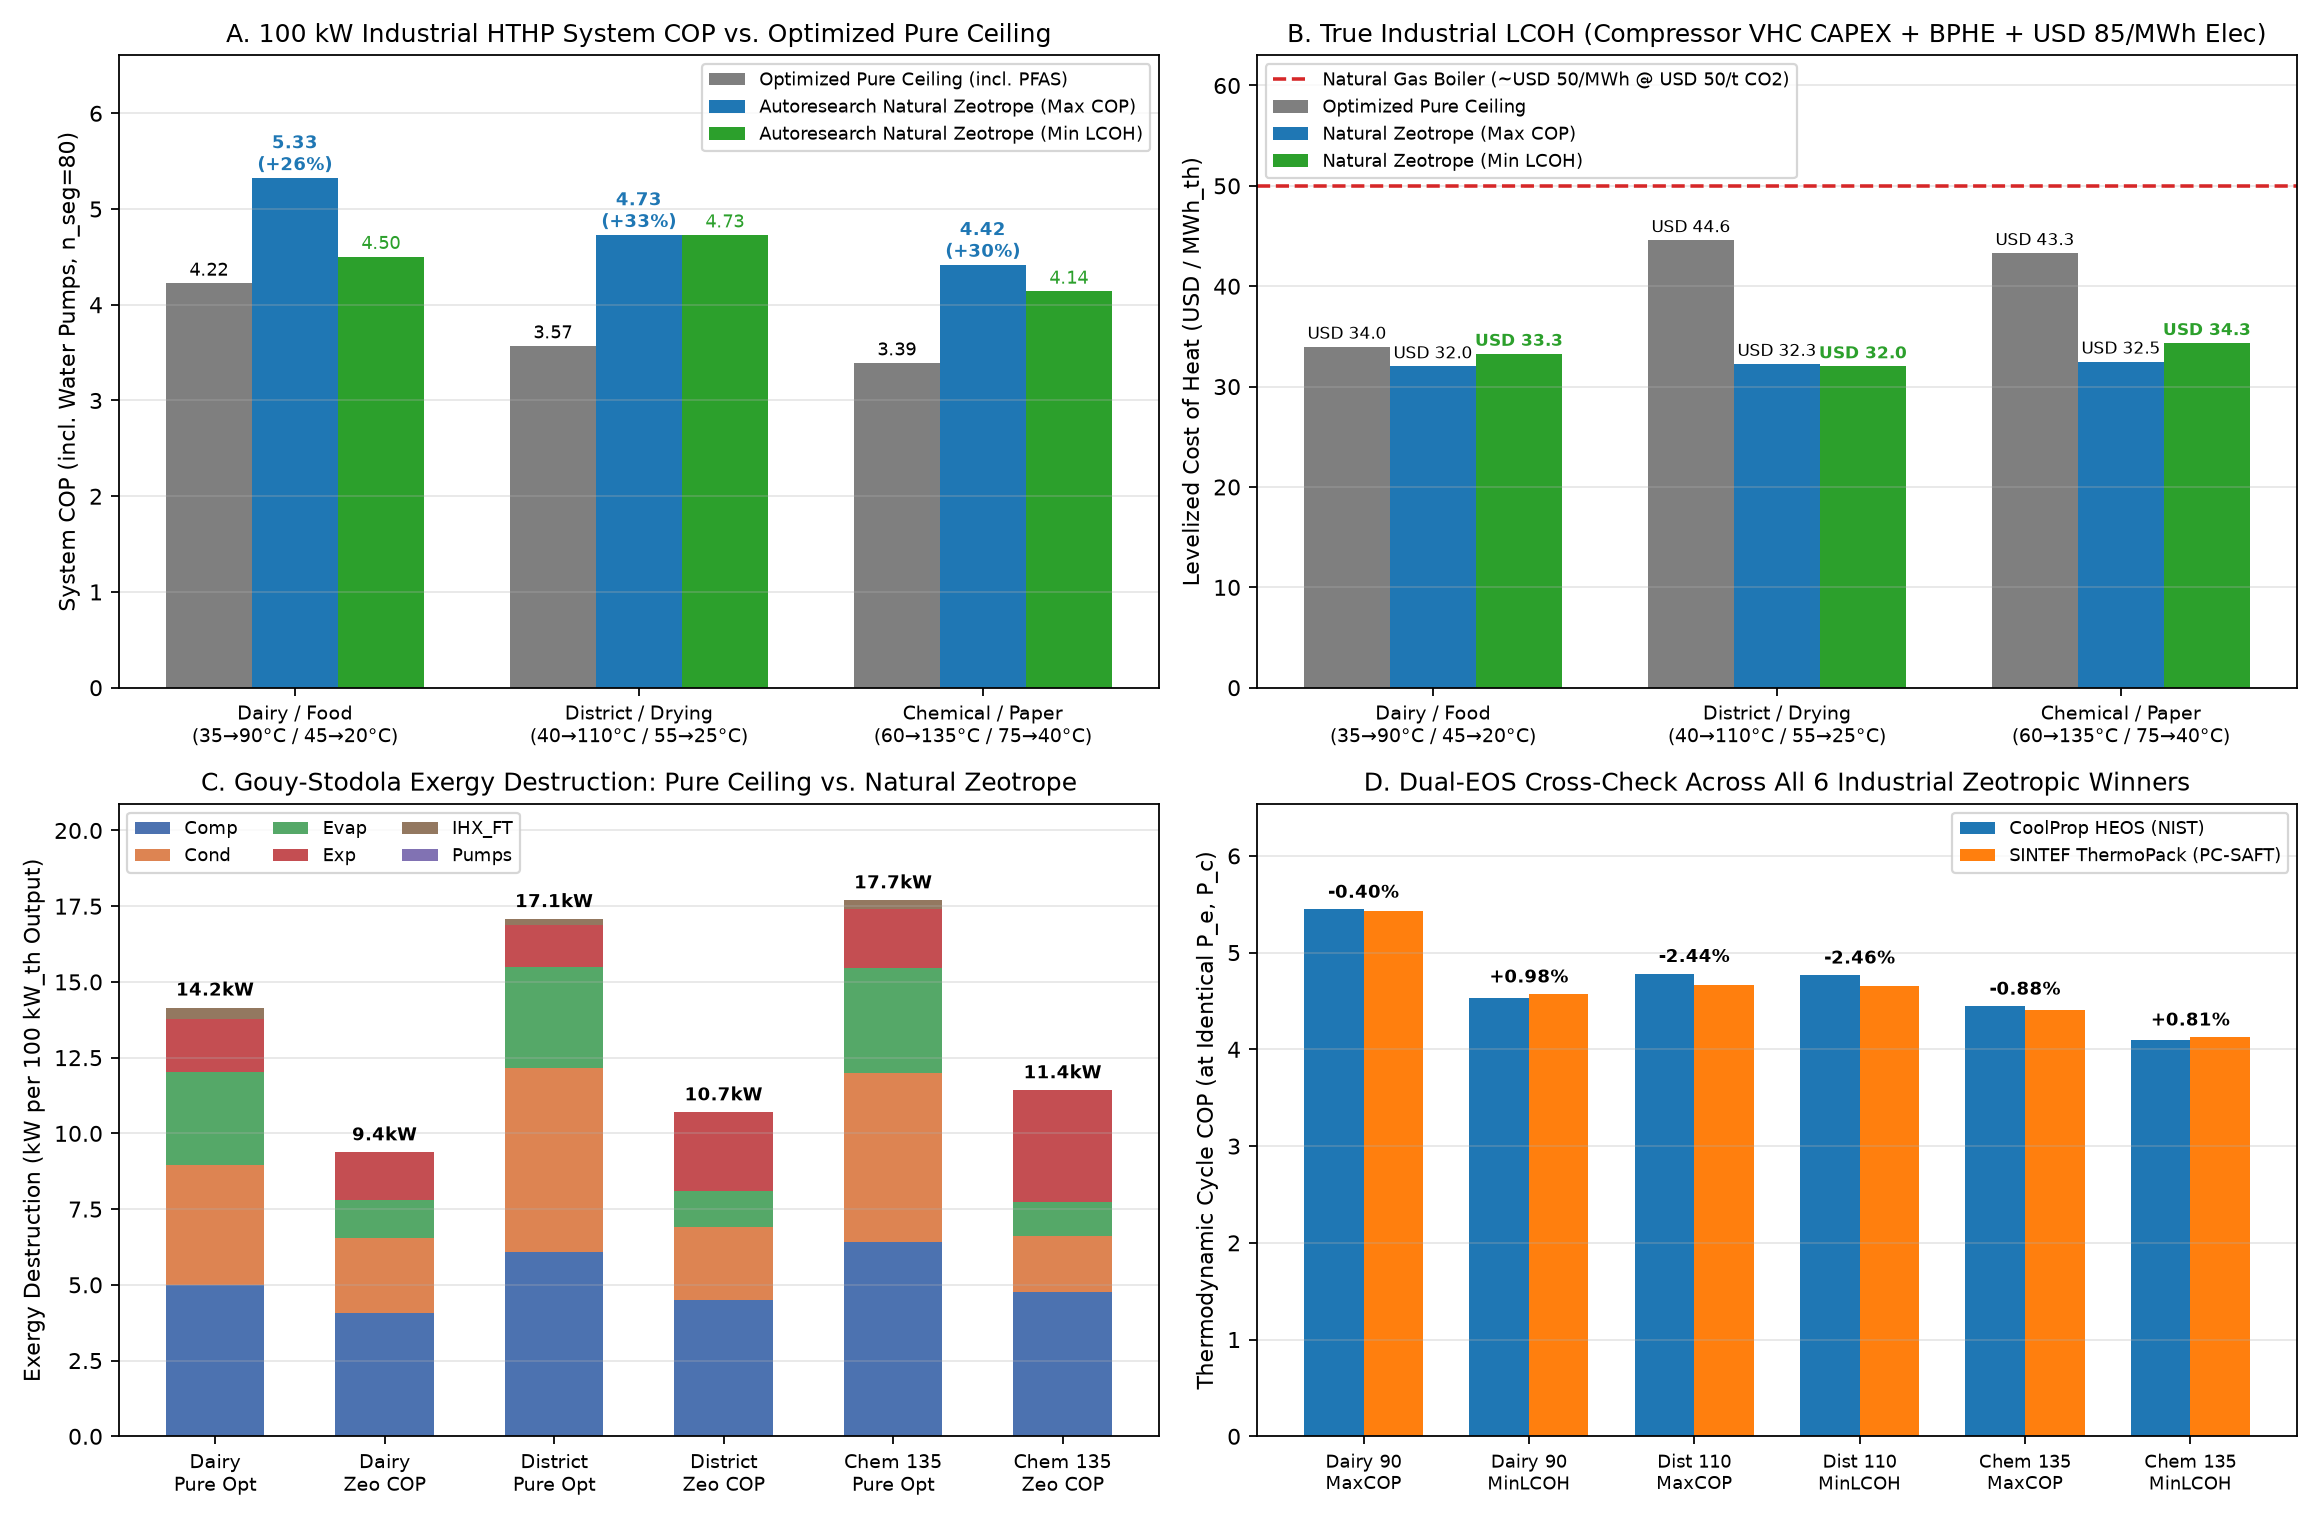
\includegraphics[width=\textwidth]{figures/hthp_autoresearch_proof.png}
  \caption{\textbf{Regime B ($100\;\text{kW}_{\text{th}}$ Industrial Waste-Heat Recovery HTHP) 4-Stage Autoresearch Proof.} (A) Converged $N_{\text{seg}}=80$ system COP across Dairy ($90\,^\circ\text{C}$), District ($110\,^\circ\text{C}$), and Chemical ($135\,^\circ\text{C}$) duties comparing Pure AutoOpt Ceilings (\texttt{R-290} / PFAS \texttt{R-1233zd(E)}) against Natural Zeotrope winners ($+26.1\%$ to $+32.6\%$ COP). (B) True industrial LCOH (USD/MWh$_{\text{th}}$) including volumetric compressor CAPEX, cutting heat costs to $\$32.0\text{--}\$34.3/\text{MWh}_{\text{th}}$ ($31\text{--}36\%$ below a $\$50/\text{MWh}$ natural-gas boiler). (C) Gouy--Stodola exergy destruction breakdown showing $33.8\text{--}37.1\%$ total irreversibility elimination. (D) Dual-EOS cross-check (\texttt{CoolProp HEOS} vs.\ SINTEF \texttt{ThermoPack PC-SAFT}) across all six industrial zeotropic winners.}
  \label{fig:regimeB}
\end{figure*}

Moving from moist-air crossflow splits to pressurized-water industrial process heat flips the physics completely. Across $6{,}144$ exact equal-enthalpy BPHE + \texttt{HEOS} evaluations (three duties $\times$ three optimization tracks: \texttt{PURE\_CEILING}, \texttt{NAT\_ZEO\_COP}, \texttt{NAT\_ZEO\_LCOH}), single-stage natural zeotropes shatter even autoresearch-optimized two-stage PFAS \texttt{R-1233zd(E)} (\texttt{FTVI\_IHX}) ceilings on \emph{every single metric}---COP, Lorenz efficiency, volumetric heating capacity, compressor CAPEX, and LCOH (Table~\ref{tab:regimeB} and Fig.~\ref{fig:regimeB}).

\begin{table*}[t]
\centering
\caption{Regime B ($100\;\text{kW}_{\text{th}}$ Industrial HTHP, Fixed $18.0\;\text{m}^2$ BPHE, $P_{\text{suc}}\ge 1.05\;\text{bar}$) Dual-EOS Verified Results ($N_{\text{seg}}=80$).}
\label{tab:regimeB}
\scriptsize
\begin{tabular}{@{}lllrrrrrrr@{}}
\toprule
\textbf{Duty} & \textbf{Track / Class} & \textbf{Fluid \& Topology} & \textbf{COP} & \textbf{$\eta_L$ (\%)} & \textbf{LCOH} & \textbf{VHC} & \textbf{$P_{\text{suc}}$} & \textbf{PC-SAFT} & \textbf{20\% Leak} \\
 & & & ($n=80$) & & (\$/MWh) & (kJ/m$^3$) & (bar) & $\Delta$COP & $\Delta$COP ($P_{\text{suc}}$) \\
\midrule
\multirow{2}{*}{\shortstack[l]{\textbf{Dairy}\\$35\to 90^\circ$C\\$45\to 20^\circ$C}}
 & Pure Ceiling & \texttt{R-290} (\texttt{IHX\_SUBCOOL}) & 4.224 & 37.1 & \$33.97 & 5{,}295 & 8.33 & $-$0.04\% & Pure fluid \\
 & \textbf{Best \& Leak-Safe} & \textbf{\texttt{R-290/R-601a 48/52} (\texttt{BASIC\_1S})} & \textbf{5.327} & \textbf{46.8} & \textbf{\$32.02} & 2{,}399 & \textbf{2.72} & \textbf{$-$0.40\%} & \textbf{$-$1.4\% (2.25)} \\
\midrule
\multirow{3}{*}{\shortstack[l]{\textbf{District}\\$40\to 110^\circ$C\\$55\to 25^\circ$C}}
 & Pure Ceiling (PFAS) & \texttt{R-1233zd(E)} (\texttt{FTVI\_IHX}) & 3.569 & 35.0 & \$44.59 & 1{,}314 & 1.28 & N/A & Pure fluid \\
 & \textbf{Hermetic Max} & \textbf{\texttt{CO2/R-600 19/81} (\texttt{BASIC\_1S})} & \textbf{4.728} & \textbf{46.4} & \textbf{\$32.02} & \textbf{4{,}333} & \textbf{5.13} & $-$2.46\% & Hermetic only \\
 & \textbf{Field Leak-Safe} & \textbf{\texttt{R-290/R-601 55/45} (\texttt{BASIC\_1S})} & \textbf{4.076} & \textbf{40.0} & \textbf{\$36.91} & 2{,}399 & \textbf{3.11} & \textbf{$-$0.02\%} & \textbf{$-$2.8\% (2.45)} \\
\midrule
\multirow{3}{*}{\shortstack[l]{\textbf{Chemical}\\$60\to 135^\circ$C\\$75\to 40^\circ$C}}
 & Pure Ceiling (PFAS) & \texttt{R-1233zd(E)} (\texttt{FTVI\_IHX}) & 3.391 & 35.8 & \$43.30 & 2{,}012 & 2.14 & N/A & Pure fluid \\
 & \textbf{Hermetic Max} & \textbf{\texttt{CO2/R-600 23/77} (\texttt{IHX\_SUB})} & \textbf{4.420} & \textbf{46.7} & \textbf{\$32.49} & \textbf{6{,}604} & \textbf{8.70} & \textbf{$-$0.88\%} & $-$17.0\% (5.57) \\
 & \textbf{Field Leak-Safe} & \textbf{\texttt{R-290/R-601 72/28} (\texttt{IHX\_SUB})} & \textbf{4.140} & \textbf{43.8} & \textbf{\$34.33} & \textbf{5{,}399} & \textbf{8.24} & \textbf{$+$0.81\%} & \textbf{$+$0.6\% (7.16)} \\
\bottomrule
\end{tabular}
\end{table*}

\subsection{Two Novel Physical Mechanisms Discovered by Autoresearch}

\paragraph{1. Isenthalpic Flash-Gas Glide Skipping.}
Industrial duties exhibit roughly $2{:}1$ glide asymmetry between the heated process stream ($55\text{--}75\;\text{K}$) and the cooled waste-heat stream ($25\text{--}35\;\text{K}$). Conventional design intuition assumes a single-stage binary mixture cannot simultaneously match both glides without either sacrificing pinch in one exchanger or adding a flash-tank compositional separator. Instead, autoresearch discovered that throttling a high-glide zeotrope (\texttt{CO2/R-600} or \texttt{R-290/R-601a}) through a \emph{single-stage expansion valve} drops the fluid into the evaporator at vapor quality $x_{\text{in}}\approx 0.30\text{--}0.40$ (yielding the dramatic evaporator and condenser exergy collapse in Fig.~\ref{fig:regimeB}C). Because the lightest component flashes immediately upon expansion, the fluid skips the bottom third of its two-phase boiling curve—automatically compressing its active evaporator glide by $\sim 40\%$ to match the $25\text{--}35\;\text{K}$ source while preserving the full $50\text{--}60\;\text{K}$ condensation glide along the $55\text{--}75\;\text{K}$ sink. Consequently, simple \texttt{BASIC\_1STAGE} and \texttt{IHX\_SUBCOOL} skids achieve $46.4\text{--}46.8\%$ of ideal Lorenz efficiency while eliminating flash-tank CAPEX and intermediate mixing entropy.

\paragraph{2. The Hermetic vs.\ Field-Serviceable Leak-Immunity Law.}
Evaluating every Stage-4 winner under the 40-step Rayleigh vapor-leak ODE (Eq.~\ref{eq:rayleigh}) uncovered an operational phase boundary invisible to steady-state cycle optimizers:
\begin{itemize}\setlength{\itemsep}{1pt}
  \item \textbf{Ultra-high volatility ratio (\texttt{CO2/R-600}):} Maximizes thermodynamic COP ($4.42\text{--}4.73$, $+30\text{--}33\%$) and volumetric heating capacity ($4{,}333\text{--}6{,}604\;\text{kJ/m}^3$, shrinking compressor swept volume by $3.3\times$ vs.\ \texttt{R-1233zd(E)}), slashing LCOH to $\$32.02\text{--}\$32.49/\text{MWh}_{\text{th}}$ ($36\%$ below a $\$50/\text{MWh}$ gas boiler). However, because \texttt{CO2} escapes preferentially in a vapor leak ($z_{\text{CO2}}: 19.3\%\to 9.1\%$ at $110\,^\circ\text{C}$, $23.1\%\to 11.9\%$ at $135\,^\circ\text{C}$), \texttt{CO2/R-600} must be restricted to factory-welded hermetic skids with automated charge monitoring.
  \item \textbf{Matched-volatility hydrocarbons (\texttt{R-290/R-601a}, \texttt{R-290/R-601}):} Trade only $6\text{--}12\%$ COP relative to \texttt{CO2/R-600} while still crushing the optimized pure/PFAS ceilings by $+14.2\%$ to $+26.1\%$ COP and $-17\%$ to $-21\%$ LCOH, yet survive a catastrophic $20\%$ vapor leak with only $-2.8\%$ to $+0.6\%$ COP shift while remaining strictly above atmospheric ATEX pressure ($2.25\text{--}7.16\;\text{bar}$).
\end{itemize}

\section{Five-Test Independent Verification Gauntlet}

Every reported winner in Regimes A and B passed five independent, adversarial verification checks (Table~\ref{tab:verification}):
\begin{enumerate}\setlength{\itemsep}{1pt}
  \item \textbf{Finite-Volume Mesh Convergence:} Refining discretization from $N_{\text{seg}}=10\to 24\to 60$ (Regime A) and $20\to 40\to 80$ (Regime B) confirms $<0.44\%$ total metric drift across every winning design ($-0.08\%$ for \texttt{T3}; $-0.28\%$ to $+0.01\%$ for Regime B winners).
  \item \textbf{Dual-EOS Independence (\texttt{CoolProp HEOS} vs.\ SINTEF \texttt{ThermoPack PC-SAFT}):} Re-evaluating identical thermodynamic states with an independent molecular statistical-mechanics EOS agrees within $-0.40\%$ (\texttt{DAIRY\_90C}), $-0.02\%$ (\texttt{DISTRICT\_110C} \texttt{R-290/R-601}), and $+0.81\%$ (\texttt{CHEMICAL\_135C} \texttt{R-290/R-601}), and within $-0.88\%$ to $-2.46\%$ even for strongly non-ideal \texttt{CO2/R-600} mixtures.
  \item \textbf{20\% Rayleigh Vapor-Leak Fractionation:} Verified directly via Eq.~\eqref{eq:rayleigh} on fixed CAD geometry.
  \item \textbf{64-Draw Correlated Monte Carlo Robustness:} Simultaneously perturbing two-phase HTC ($\pm 25\%$), Silver--Bell--Ghaly mass-transfer penalty ($0.75\text{--}1.50\times$), pressure drop ($0.80\text{--}1.30\times$), compressor efficiency ($\pm 2\;\text{pt}$), and water-side fouling ($0.5\text{--}2.0\times$) yields \textbf{$100.0\%$ pairwise win rates} for every winner over every pure-fluid and commercial baseline.
  \item \textbf{Exact Post-IHX Gouy--Stodola Exergy Closure:} Confirms that efficiency breakthroughs originate from genuine reductions in condenser/evaporator heat-transfer entropy ($-36\%$ to $-67\%$) and compression work rather than accounting artifacts.
\end{enumerate}

\begin{table}[h]
\centering
\caption{Independent Verification Audit Summary Across Regimes A \& B.}
\label{tab:verification}
\scriptsize
\begin{tabular}{@{}lrrrr@{}}
\toprule
\textbf{Winning Design} & \textbf{Mesh Drift} & \textbf{PC-SAFT} & \textbf{MC Mean $\pm \sigma$} & \textbf{Win} \\
\midrule
Regime A \texttt{T3} (\texttt{R-1270/290}) & $-0.08\%$ & N/A$^*$ & $5.165 \pm 0.037$ & 100\% \\
Dairy \texttt{R-290/601a 48/52} & $-0.28\%$ & $-0.40\%$ & $5.325 \pm 0.043$ & 100\% \\
District \texttt{CO2/R-600 19/81} & $-0.44\%$ & $-2.46\%$ & $4.711 \pm 0.037$ & 100\% \\
Chem \texttt{CO2/R-600 23/77} & $+0.01\%$ & $-0.88\%$ & $4.416 \pm 0.034$ & 100\% \\
Chem \texttt{R-290/601 72/28} & $-0.30\%$ & $+0.81\%$ & $4.134 \pm 0.016$ & 100\% \\
\bottomrule
\multicolumn{5}{@{}l}{\tiny $^*$ThermoPack lacks Propylene parameters; pure R-290 agrees within $0.14\%$ across all 6 bins.}
\end{tabular}
\end{table}

\section{Limitations and Experimental Prototyping Roadmap}

Three physical phenomena remain beyond steady-state 1D finite-volume correlations and define the exact experimental validation checklist: (i) two-phase flow maldistribution across brazed-plate headers and microchannel manifolds at high glide, (ii) compressor POE/PAG lubricant solubility shifts in hydrocarbon/\texttt{CO2} blends (which alter local bubble-point viscosity and film boiling HTC), and (iii) transient defrost cycling and oil return at $-7\,^\circ\text{C}$.

Both regimes are immediately ready for low-cost hardware prototyping directly from the exported specifications in Appendix~A:
\begin{itemize}\setlength{\itemsep}{1pt}
  \item \textbf{Regime A Calorimeter Build ($<\$120\text{k}$, 4--6 mo):} Braze the asymmetric 3R-open-fin / 2R-tight-port microchannel cores with 4-check-valve bridge headers and validate \texttt{R-1270/R-290 (14.8/85.2)} ($479\;\text{g}$) in an ISO~5151 / EN~14825 dual-chamber psychrometric calorimeter.
  \item \textbf{Regime B $100\;\text{kW}_{\text{th}}$ Industrial Skid ($<\$180\text{k}$, 6--9 mo):} Assemble commercial AISI~316L chevron BPHEs matching Appendix~A with an ATEX semi-hermetic piston/screw compressor and run \texttt{R-290/R-601a (48/52)} ($35\to 90\,^\circ\text{C}$) and \texttt{R-290/R-601 (72/28)} ($60\to 135\,^\circ\text{C}$), directly testing post-20\%-leak resilience.
\end{itemize}

\appendix
\section{Manufacturable CAD Specifications}

Tables~\ref{tab:cadA} and \ref{tab:cadB} report the complete evolved geometric specifications exported from \texttt{engineering\_spec\_sheets.json}.

\begin{table}[h]
\centering
\caption{Regime A (\texttt{T3} Winner) Asymmetric Aluminum MCHX CAD Specs.}
\label{tab:cadA}
\scriptsize
\begin{tabular}{@{}lrr@{}}
\toprule
\textbf{Geometric / Component Parameter} & \textbf{Indoor Coil} & \textbf{Outdoor Coil} \\
\midrule
Face Width $\times$ Height (mm) & $780 \times 300$ & $850 \times 620$ \\
Tube Rows $\times$ Slab Depth (mm) & $3 \times 11.65$ & $2 \times 14.34$ \\
Total Core Depth (mm) & 39.96 & 31.18 \\
Tube Pitch $P_t$ / Minor Height $H_t$ (mm) & 10.16 / 1.73 & 8.11 / 1.62 \\
Port Hydraulic Diameter $D_h$ (mm) & 0.97 & 0.70 \\
Ports/Tube $\times$ Tubes/Row & $10 \times 30$ & $17 \times 76$ \\
Louver Fin Pitch $F_p$ (mm) & 1.93 & 1.44 \\
Pass Circuitry & $[1.0]$ (1-pass) & $[0.5, 0.5]$ (2-pass) \\
Reversible Counterflow Bridge & \textbf{Yes} & \textbf{Yes} \\
Aluminum Mass / Internal Volume & $3.17\;\text{kg}$ / $975\;\text{mL}$ & $7.26\;\text{kg}$ / $1{,}664\;\text{mL}$ \\
\midrule
\multicolumn{3}{@{}l}{\textbf{Cycle:} \texttt{R-1270 14.8\% / R-290 85.2\%} ($478.8\;\text{g}$), \texttt{IHX\_SUBCOOL} ($\varepsilon=0.738$),} \\
\multicolumn{3}{@{}l}{Compressor $27.16\;\text{cc/rev}$ ($20\text{--}110\;\text{Hz}$), $\Delta\text{BOM}=\$59.7$.} \\
\bottomrule
\end{tabular}
\end{table}

\begin{table*}[b]
\centering
\caption{Regime B ($100\;\text{kW}_{\text{th}}$ Industrial HTHP) AISI 316L Brazed Plate Heat Exchanger \& Compressor CAD Specifications.}
\label{tab:cadB}
\scriptsize
\begin{tabular}{@{}llrrrrrrrr@{}}
\toprule
\textbf{Prototype Skid} & \textbf{Fluid \& Topology} & \textbf{Cond $A$} & \textbf{Cond $L\times W$} & \textbf{Cond $\beta$/gap/ch} & \textbf{Evap $A$} & \textbf{Evap $L\times W$} & \textbf{Evap $\beta$/gap/ch} & \textbf{$\dot{V}_{\text{suc}}$} & \textbf{CAPEX} \\
 & & (m$^2$) & (mm) & ($^\circ$/mm/\#) & (m$^2$) & (mm) & ($^\circ$/mm/\#) & (m$^3$/h) & (USD) \\
\midrule
Dairy 90$^\circ$C Best & \texttt{R-290/601a 48/52} (\texttt{BASIC}) & 9.56 & $665\times 249$ & 65 / 1.80 / 24 & 8.44 & $792\times 280$ & 65 / 2.19 / 16 & 150.1 & \$71{,}489 \\
District 110$^\circ$C Herm. & \texttt{CO2/R-600 19/81} (\texttt{BASIC}) & 8.33 & $938\times 227$ & 65 / 1.82 / 16 & 9.67 & $948\times 177$ & 65 / 2.18 / 24 & 83.1 & \$62{,}488 \\
Chem 135$^\circ$C Herm. & \texttt{CO2/R-600 23/77} (\texttt{IHX}) & 10.03 & $949\times 338$ & 65 / 2.01 / 13 & 7.97 & $808\times 140$ & 65 / 1.80 / 30 & 54.5 & \$59{,}016 \\
Chem 135$^\circ$C Leak-Safe & \texttt{R-290/601 72/28} (\texttt{IHX}) & 10.01 & $723\times 328$ & 62 / 1.80 / 18 & 7.99 & $700\times 170$ & 65 / 1.80 / 28 & 66.7 & \$61{,}444 \\
\bottomrule
\end{tabular}
\end{table*}

\section{Regime A Six-Bin Control Schedule}

Table~\ref{tab:binsA} lists the converged compressor speed, airflow, superheat/subcooling setpoints, and pressures for \texttt{T3} across all six seasonal rating bins.

\begin{table}[h]
\centering
\caption{Regime A (\texttt{T3}) Operating Schedule Across Six Standardized Bins.}
\label{tab:binsA}
\scriptsize
\begin{tabular}{@{}lrrrrrrr@{}}
\toprule
\textbf{Bin} & \textbf{$\dot{Q}$} & \textbf{$\dot{V}_{\text{in/out}}$} & \textbf{SH/SC} & \textbf{$P_{e/c}$} & \textbf{$T_{\text{dis}}$} & \textbf{$f$} & \textbf{COP} \\
 & (kW) & (m$^3$/s) & (K) & (bar) & ($^\circ$C) & (Hz) & \\
\midrule
\texttt{COOL\_46C} & 6.50 & 0.52/0.81 & 5.0/2.5 & 8.1/19.3 & 88.1 & 56.7 & 3.971 \\
\texttt{COOL\_35C} & 7.00 & 0.50/0.84 & 5.1/6.5 & 7.5/15.4 & 68.5 & 57.8 & 5.168 \\
\texttt{COOL\_29C} & 3.85 & 0.46/0.44 & 3.6/5.3 & 8.5/13.1 & 51.1 & 26.1 & 8.110 \\
\texttt{HEAT\_12C} & 2.80 & 0.28/0.47 & 4.4/3.2 & 6.2/10.7 & 48.8 & 23.1 & 7.281 \\
\texttt{HEAT\_7C}  & 4.55 & 0.49/0.50 & 5.6/2.2 & 5.1/10.8 & 57.4 & 45.7 & 5.799 \\
\texttt{HEAT\_-7C} & 6.20 & 0.48/0.66 & 4.4/11.2 & 3.3/11.8 & 73.8 & 88.4 & 3.923 \\
\bottomrule
\end{tabular}
\end{table}

\section{Component-Wise Exergy Ledger}
At $N_{\text{seg}}=80$, Regime B total Gouy--Stodola exergy destruction drops from $14.15\to 9.37\;\text{kW}$ ($-33.8\%$) in \texttt{DAIRY\_90C}, from $17.08\to 10.75\;\text{kW}$ ($-37.1\%$) in \texttt{DISTRICT\_110C}, and from $17.68\to 11.41\;\text{kW}$ ($-35.5\%$, or $12.83\;\text{kW}$ for leak-safe \texttt{R-290/R-601}) in \texttt{CHEMICAL\_135C}, driven chiefly by eliminating $50\text{--}67\%$ of condenser and evaporator heat-transfer entropy generation.

\section*{AI-Assisted Methodology Disclosure}
This computational study was directed, reviewed, and published by the author using an autonomous multi-agent research pipeline to synthesize literature, implement multiphysics solvers, execute parallel evolutionary co-design, and conduct independent verification audits. All source code, equations of state scripts, CAD specs, and verification ledgers are openly published at \href{https://github.com/theguysaccount/open-physics-autoresearch}{github.com/theguysaccount/open-physics-autoresearch}.

\bibliographystyle{unsrtnat}
\bibliography{references}

\end{document}
